% Low-fidelity wireframes of the main screens
\tikzset{
  frame/.style={draw=black!70, thick, fill=white},
  blk/.style={draw=black!50, fill=black!8},
  blkd/.style={draw=black!55, fill=black!18},
  wtxt/.style={font=\tiny, text=black!70},
  btn/.style={draw=black!60, fill=black!25, rounded corners=1.5pt, font=\tiny, inner sep=1.5pt},
}
% navbar: \navbar{width}{height-of-frame}
\newcommand{\wfnavbar}[2]{%
  \draw[blkd] (0,#2-0.6) rectangle (#1,#2);
  \node[wtxt, font=\scriptsize\bfseries, anchor=west] at (0.15,#2-0.3) {TalkCS};
  \draw[blk, fill=white] (#1*0.30,#2-0.45) rectangle (#1*0.62,#2-0.15);
  \node[wtxt, anchor=west] at (#1*0.31,#2-0.3) {Search...};
  \node[btn] at (#1*0.70,#2-0.3) {+ Create Post};
  \foreach \k in {0,1,2,3} {\draw[black!60] (#1*0.80+\k*0.42,#2-0.3) circle (0.12);}
}

\begin{figure}[H]
  \centering
  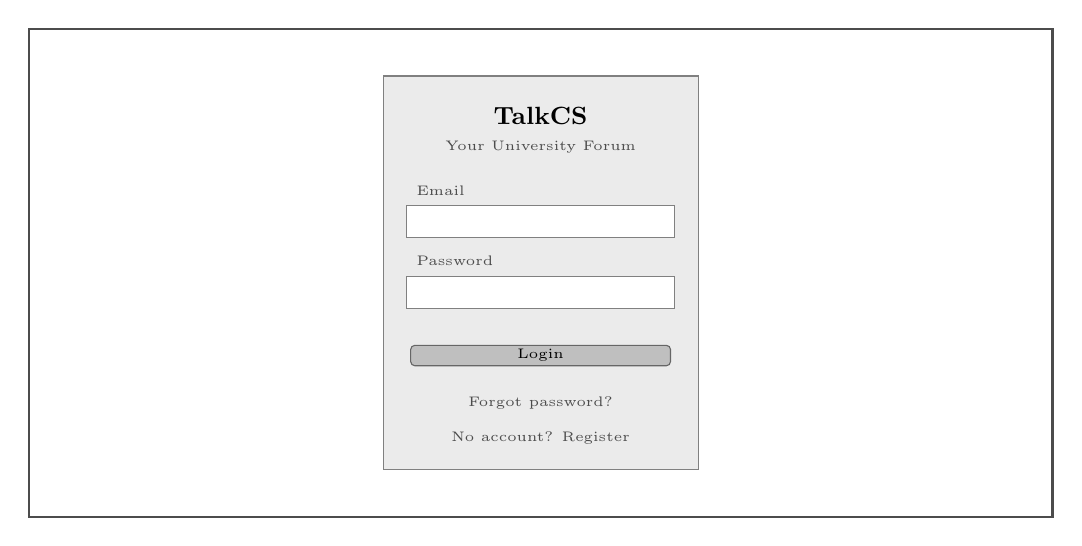
\begin{tikzpicture}[scale=1]
    \draw[frame] (0,0) rectangle (13,6.2);
    \draw[blk] (4.5,0.6) rectangle (8.5,5.6);
    \node[font=\small\bfseries] at (6.5,5.1) {TalkCS};
    \node[wtxt] at (6.5,4.7) {Your University Forum};
    \node[wtxt, anchor=west] at (4.8,4.15) {Email};
    \draw[fill=white, draw=black!50] (4.8,3.55) rectangle (8.2,3.95);
    \node[wtxt, anchor=west] at (4.8,3.25) {Password};
    \draw[fill=white, draw=black!50] (4.8,2.65) rectangle (8.2,3.05);
    \node[btn, minimum width=3.3cm] at (6.5,2.05) {Login};
    \node[wtxt] at (6.5,1.45) {Forgot password?};
    \node[wtxt] at (6.5,1.0) {No account? Register};
  \end{tikzpicture}
  \caption{Wireframe of the Login page}
  \label{fig:wf-login}
\end{figure}

\begin{figure}[H]
  \centering
  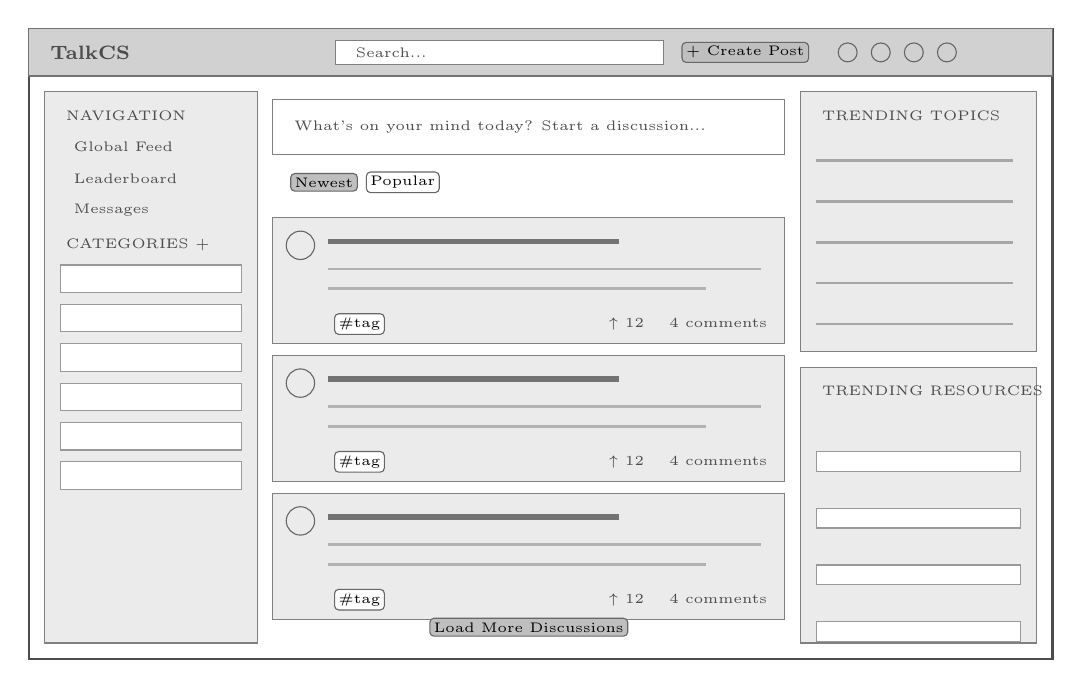
\begin{tikzpicture}
    \draw[frame] (0,0) rectangle (13,8);
    \wfnavbar{13}{8}
    % left sidebar
    \draw[blk] (0.2,0.2) rectangle (2.9,7.2);
    \node[wtxt, anchor=west] at (0.35,6.9) {NAVIGATION};
    \foreach \t [count=\i] in {Global Feed, Leaderboard, Messages} {\node[wtxt, anchor=west] at (0.45,6.9-\i*0.4) {\t};}
    \node[wtxt, anchor=west] at (0.35,5.25) {CATEGORIES \hfill +};
    \foreach \i in {1,...,6} {\draw[black!40, fill=white] (0.4,5.15-\i*0.5) rectangle (2.7,5.5-\i*0.5);}
    % center feed
    \draw[blk, fill=white] (3.1,6.4) rectangle (9.6,7.1);
    \node[wtxt, anchor=west] at (3.25,6.75) {What's on your mind today? Start a discussion...};
    \node[btn] at (3.75,6.05) {Newest}; \node[btn, fill=white] at (4.75,6.05) {Popular};
    \foreach \i in {0,1,2} {
      \draw[blk] (3.1,4.0-\i*1.75) rectangle (9.6,5.6-\i*1.75);
      \draw[black!60] (3.45,5.25-\i*1.75) circle (0.18);
      \draw[black!55, line width=2pt] (3.8,5.3-\i*1.75) -- (7.5,5.3-\i*1.75);
      \draw[black!30, line width=1pt] (3.8,4.95-\i*1.75) -- (9.3,4.95-\i*1.75);
      \draw[black!30, line width=1pt] (3.8,4.7-\i*1.75) -- (8.6,4.7-\i*1.75);
      \node[btn, fill=white] at (4.2,4.25-\i*1.75) {\#tag};
      \node[wtxt, anchor=east] at (9.5,4.25-\i*1.75) {$\uparrow$ 12 \quad 4 comments};
    }
    \node[btn] at (6.35,0.4) {Load More Discussions};
    % right sidebar
    \draw[blk] (9.8,3.9) rectangle (12.8,7.2);
    \node[wtxt, anchor=west] at (9.95,6.9) {TRENDING TOPICS};
    \foreach \i in {1,...,5} {\draw[black!35, line width=1pt] (10.0,6.85-\i*0.52) -- (12.5,6.85-\i*0.52);}
    \draw[blk] (9.8,0.2) rectangle (12.8,3.7);
    \node[wtxt, anchor=west] at (9.95,3.4) {TRENDING RESOURCES};
    \foreach \i in {1,...,4} {\draw[black!40, fill=white] (10.0,3.35-\i*0.72) rectangle (12.6,2.85-\i*0.72+0.25);}
  \end{tikzpicture}
  \caption{Wireframe of the Home page}
  \label{fig:wf-home}
\end{figure}

\begin{figure}[H]
  \centering
  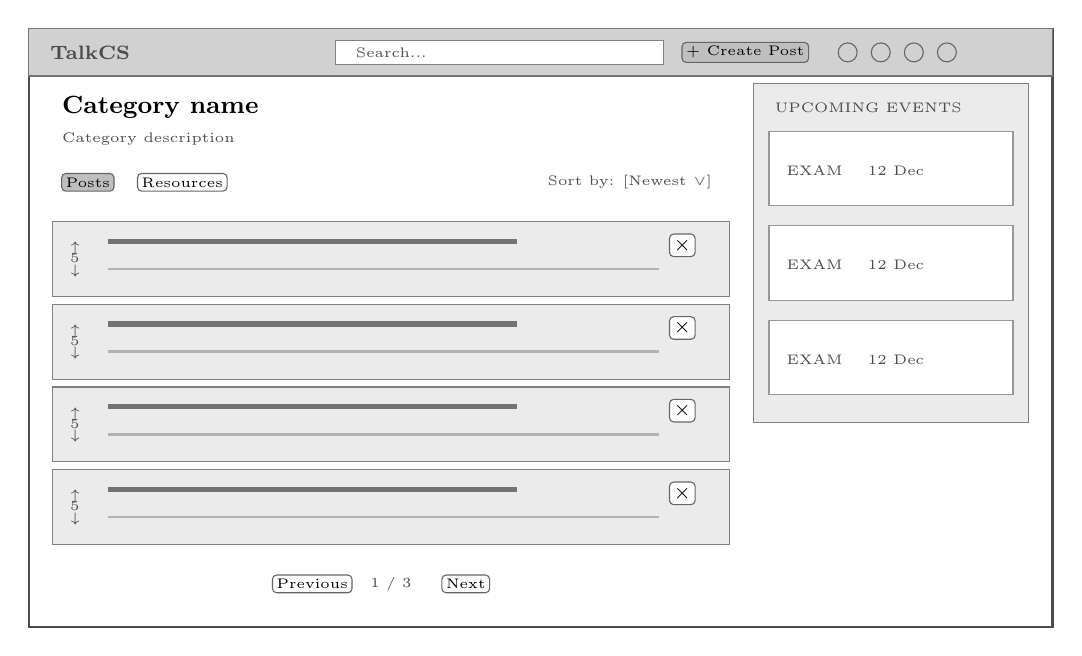
\begin{tikzpicture}
    \draw[frame] (0,0) rectangle (13,7.6);
    \wfnavbar{13}{7.6}
    \node[font=\small\bfseries, anchor=west] at (0.3,6.6) {Category name};
    \node[wtxt, anchor=west] at (0.3,6.2) {Category description};
    \node[btn] at (0.75,5.65) {Posts}; \node[btn, fill=white] at (1.95,5.65) {Resources};
    \node[wtxt, anchor=east] at (8.8,5.65) {Sort by: [Newest $\vee$]};
    \foreach \i in {0,1,2,3} {
      \draw[blk] (0.3,4.2-\i*1.05) rectangle (8.9,5.15-\i*1.05);
      \node[wtxt, anchor=west, align=left] at (0.4,4.67-\i*1.05) {$\uparrow$\\[-2pt]5\\[-2pt]$\downarrow$};
      \draw[black!55, line width=2pt] (1.0,4.9-\i*1.05) -- (6.2,4.9-\i*1.05);
      \draw[black!30, line width=1pt] (1.0,4.55-\i*1.05) -- (8.0,4.55-\i*1.05);
      \node[btn, fill=white] at (8.3,4.85-\i*1.05) {\scriptsize$\times$};
    }
    \node[btn, fill=white] at (3.6,0.55) {Previous}; \node[wtxt] at (4.6,0.55) {1 / 3}; \node[btn, fill=white] at (5.55,0.55) {Next};
    \draw[blk] (9.2,2.6) rectangle (12.7,6.9);
    \node[wtxt, anchor=west] at (9.35,6.6) {UPCOMING EVENTS};
    \foreach \i in {1,2,3} {\draw[black!40, fill=white] (9.4,6.55-\i*1.2) rectangle (12.5,6.55-\i*1.2+0.95);
      \node[wtxt, anchor=west] at (9.5,6.55-\i*1.2+0.45) {EXAM \quad 12 Dec};}
  \end{tikzpicture}
  \caption{Wireframe of the Category page}
  \label{fig:wf-category}
\end{figure}

\begin{figure}[H]
  \centering
  \begin{tikzpicture}
    \draw[frame] (0,0) rectangle (13,9);
    \wfnavbar{13}{9}
    \draw[blk] (0.3,5.2) rectangle (12.7,8.2);
    \node[wtxt, anchor=west, align=left] at (0.45,7.0) {$\uparrow$\\[-1pt]\small 12\\[-1pt]$\downarrow$};
    \draw[black!60, line width=3pt] (1.2,7.8) -- (8.0,7.8);
    \node[btn, fill=tcgreen] at (8.8,7.8) {SOLVED};
    \node[wtxt, anchor=west] at (1.2,7.45) {author \textbullet{} Lv.3 Regular \textbullet{} 2 days ago};
    \foreach \y in {7.0,6.7,6.4} {\draw[black!30, line width=1pt] (1.2,\y) -- (12.2,\y);}
    \draw[black!50, fill=black!12] (1.2,5.5) rectangle (8.0,6.2); \node[wtxt] at (4.6,5.85) {code block};
    \node[btn, fill=white] at (9.0,5.55) {\#java}; \node[btn, fill=white] at (10.0,5.55) {\#spring};
    \node[wtxt] at (12.3,7.8) {$\square$};
    \node[font=\scriptsize\bfseries, anchor=west] at (0.3,4.8) {Comments};
    \draw[fill=white, draw=black!50] (0.3,4.0) rectangle (12.7,4.5); \node[wtxt, anchor=west] at (0.4,4.25) {Write a comment...};
    \draw[blk, fill=tcgreen!50] (0.3,2.6) rectangle (12.7,3.75);
    \node[wtxt, anchor=west] at (0.4,3.5) {\checkmark{} Accepted Answer \quad answerer \textbullet{} Lv.2};
    \draw[black!30, line width=1pt] (0.9,3.1) -- (11.5,3.1);
    \node[wtxt, anchor=west] at (0.4,2.8) {$\uparrow$ 4 $\downarrow$ \quad Reply};
    \draw[blk] (1.3,1.5) rectangle (12.7,2.4);
    \draw[black!30, line width=1pt] (1.6,2.05) -- (11.0,2.05);
    \node[wtxt, anchor=west] at (1.4,1.7) {$\uparrow$ 1 $\downarrow$ \quad Reply \quad (nested reply)};
    \draw[blk] (0.3,0.3) rectangle (12.7,1.3);
    \draw[black!30, line width=1pt] (0.9,0.9) -- (11.0,0.9);
  \end{tikzpicture}
  \caption{Wireframe of the Post page}
  \label{fig:wf-post}
\end{figure}

\begin{figure}[H]
  \centering
  \begin{tikzpicture}
    \draw[frame] (0,0) rectangle (13,7.2);
    \wfnavbar{13}{7.2}
    \draw[blk] (0.2,0.2) rectangle (4.2,6.4);
    \node[font=\scriptsize\bfseries, anchor=west] at (0.35,6.1) {Messages};
    \draw[fill=white, draw=black!50] (0.35,5.4) rectangle (4.05,5.8); \node[wtxt, anchor=west] at (0.45,5.6) {Find user...};
    \foreach \i in {1,...,5} {
      \draw[black!40, fill=white] (0.35,5.3-\i*0.95) rectangle (4.05,5.3-\i*0.95+0.85);
      \draw[black!60] (0.7,5.3-\i*0.95+0.42) circle (0.2);
      \draw[black!55, line width=1.5pt] (1.05,5.3-\i*0.95+0.55) -- (2.6,5.3-\i*0.95+0.55);
      \draw[black!30, line width=1pt] (1.05,5.3-\i*0.95+0.27) -- (3.3,5.3-\i*0.95+0.27);
    }
    \node[circle, fill=tcorange, inner sep=1.2pt, font=\tiny, text=white] at (3.8,4.77) {2};
    \draw[blk] (4.4,0.2) rectangle (12.8,6.4);
    \draw[blkd] (4.4,5.8) rectangle (12.8,6.4); \node[wtxt, anchor=west] at (4.55,6.1) {other user};
    \foreach \y/\x/\w in {5.2/4.6/3.5, 4.5/8.9/3.7, 3.8/4.6/2.6, 3.1/9.6/3.0} {\draw[black!45, fill=white, rounded corners=3pt] (\x,\y-0.45) rectangle (\x+\w,\y);}
    \draw[fill=white, draw=black!50] (4.6,0.4) rectangle (11.9,0.95); \node[wtxt, anchor=west] at (4.7,0.67) {Type your message...};
    \node[btn] at (12.35,0.67) {$\triangleright$};
  \end{tikzpicture}
  \caption{Wireframe of the Chat page}
  \label{fig:wf-chat}
\end{figure}
